\documentclass{article}



\usepackage{arxiv}

\usepackage[utf8]{inputenc} % allow utf-8 input
\usepackage[T1]{fontenc}    % use 8-bit T1 fonts
\usepackage{hyperref}       % hyperlinks
\usepackage{url}            % simple URL typesetting
\usepackage{booktabs}       % professional-quality tables
\usepackage{amsfonts}       % blackboard math symbols
\usepackage{nicefrac}       % compact symbols for 1/2, etc.
\usepackage{microtype}      % microtypography
\usepackage{lipsum}		% Can be removed after putting your text content
\usepackage{graphicx}
\usepackage{natbib}
\usepackage{doi}
\usepackage{amsmath}
\usepackage{bm}            % bold math symbols


\title{Project Report: Fracture Fixation FEA Simulation}

%\date{September 9, 1985}	% Here you can change the date presented in the paper title
%\date{} 					% Or removing it

\author{
  Wenye Xiong \\
  2023533141 \\
  \texttt{xiongwy2023@shanghaitech.edu.cn}
  \And
  Renyi Yang \\
  2023533030 \\
  \texttt{yangry2023@shanghaitech.edu.cn}
  \AND
  Zijian Li \\
  2023533185 \\
  \texttt{lizj2023@shanghaitech.edu.cn}
	%% \AND
	%% Coauthor \\
	%% Affiliation \\
	%% Address \\
	%% \texttt{email} \\
	%% \And
	%% Coauthor \\
	%% Affiliation \\
	%% Address \\
	%% \texttt{email} \\
	%% \And
	%% Coauthor \\
	%% Affiliation \\
	%% Address \\
	%% \texttt{email} \\
}

% Uncomment to remove the date
%\date{}

% Uncomment to override  the `A preprint' in the header
\renewcommand{\headeright}{SI114H Project Report}
\renewcommand{\undertitle}{SI114H Project Report}
\renewcommand{\shorttitle}{Fracture Fixation FEA Simulation}

%%% Add PDF metadata to help others organize their library
%%% Once the PDF is generated, you can check the metadata with
%%% $ pdfinfo template.pdf
\hypersetup{
pdftitle={Fracture Fixation FEA Simulation},
pdfsubject={q-bio.NC, q-bio.QM, eng.BIO},
pdfauthor={Wenye Xiong, Renyi Yang, Zijian Li},
pdfkeywords={Finite element analysis, Fracture fixation, Bone healing, Stress transfer, Biomechanics, Callus stiffening, Fixator stiffness},
}

\begin{document}
\maketitle

\begin{abstract}
  This project utilizes Finite Element Analysis to investigate the critical biomechanical phenomenon of "stress transfer" during the fracture healing process. A 2D computational model of a "bone-fixator" system was developed to analyze how varying fixator stiffness influences stress redistribution among the bone, fixator, and nascent callus. Furthermore, the study examines the resultant strain environment within the fracture gap as the bone progressively regains its load-bearing capacity. By simulating the gradual maturation of callus tissue under different fixator rigidities, this research aims to elucidate the complex interplay between fixator mechanical properties and the evolving biomechanical conditions at the fracture site. The findings are intended to provide valuable insights for optimizing fracture fixation strategies to enhance healing outcomes.
\end{abstract}


% keywords can be removed
\keywords{Finite element analysis \and Fracture fixation \and Small deformation theory \and Stress transfer \and Fixator stiffness \and Bone healing}

\section{Introduction}

Fracture healing is a dynamic biological process profoundly influenced by its mechanical environment. A key aspect of successful osteosynthesis is the gradual transfer of physiological loads from the orthopedic fixator back to the healing bone as it regenerates and regains structural integrity. This "stress transfer" mechanism is essential for stimulating bone formation and remodeling. This project employs Finite Element Analysis, a powerful computational tool, to model and investigate this critical stress transfer phenomenon. Specifically, we developed a simplified 2D "bone-fixator" system to explore how variations in fixator stiffness affect the distribution of mechanical stresses within the bone, the fixator itself, and the developing callus tissue at the fracture site. Concurrently, we analyze the mechanical strain experienced within the fracture gap, a crucial parameter known to modulate cellular activity during healing. By simulating the progressive stiffening of the callus over time, this study aims to provide a clearer understanding of how fixator design choices impact the biomechanical milieu of a healing fracture, which is vital for optimizing clinical treatments and minimizing complications such as delayed union or non-union.

\section{Overview of existing work}

Finite Element Analysis has become an indispensable tool in biomechanical research, particularly in orthopedics, for simulating and analyzing the behavior of biological structures and medical devices under diverse physiological conditions. It plays a crucial role in understanding fracture mechanics, optimizing implant design, and predicting the efficacy of various fracture fixation strategies \citep{lewis2021finite}. Traditional evaluative methods, such as in vitro experiments and clinical trials, while essential, often present limitations regarding cost, duration, and the feasibility of extensive parametric studies. FEA offers a robust complementary approach, enabling detailed, non-invasive examination of complex stress and strain distributions within bone-implant constructs.

A central concept in fracture fixation is "stress shielding," where an overly rigid fixation device bears a disproportionate share of the applied load, thereby reducing the mechanical stimulus transmitted to the healing bone. While a degree of stress shielding is necessary for initial fracture stability, excessive shielding can impede natural bone healing by inhibiting callus formation and its subsequent remodeling into lamellar bone. Conversely, insufficient stability due to overly flexible fixation can lead to excessive interfragmentary motion, potentially resulting in hypertrophic non-union or fixation failure. Consequently, achieving an optimal mechanical environment that balances stability with appropriate mechanical stimulation is paramount for successful fracture healing.

Recent advancements in computational biomechanics have focused on developing sophisticated models that can simulate the mechanobiological processes governing fracture healing. These models often incorporate time-dependent material properties for the healing callus and consider the influence of mechanical stimuli, such as strain or hydrostatic stress, on tissue differentiation pathways \citep{morgan2024novel}. Parametric studies using FEA are instrumental in investigating how factors like fixator stiffness, fracture gap size, loading conditions, and healing progression affect the stress transfer dynamics from the fixator to the bone. This project aligns with this research trajectory by systematically investigating how different fixator stiffnesses influence stress distribution patterns and fracture gap strains throughout a simulated healing period.

\section{Integration of the content of the course}

This study leverages Finite Element Analysis to model the complex stress redistribution dynamics that occur during fracture healing. The model incorporates time-dependent material properties for the healing callus and facilitates parametric studies on the influence of fixator stiffness.

\subsection{Problem Definition}

\begin{itemize}
  \item \textbf{Domain Type}: Non-homogeneous, linear elastic body subjected to quasi-static loading, featuring time-varying material properties (specifically, the elastic modulus of the callus).
  \item \textbf{Computational Model}: A 2D plane stress representation of a "bone-fixator" system, incorporating a healing fracture gap (callus). The domain is discretized using quadrilateral finite elements.
  \item \textbf{Key Features Investigated}:
        \begin{itemize}
          \item Simulation of the progressive stress transfer from the fixator to the bone tissue as callus stiffness increases with healing.
          \item Parametric analysis of the system's response under varying fixator stiffness conditions.
          \item Quantitative evaluation of stress shielding effects imparted by the fixator.
          \item Monitoring and analysis of the evolution of strain within the fracture gap (callus region).
        \end{itemize}
\end{itemize}

\subsection{Mathematical Model}

\subsubsection{Mechanical Framework}

The problem is formulated within the context of linear elasticity, considering time-dependent material properties. The constitutive relationship is given by:
\[
  \bm{\sigma}^{(t)} = \mathbf{D}^{(t)}\bm{\varepsilon}
\]
where:
\begin{itemize}
  \item $\bm{\sigma}^{(t)}$ represents the Cauchy stress tensor at a given healing time point $t$.
  \item $\bm{\varepsilon}$ is the small strain tensor, defined as $\varepsilon_{ij} = \frac{1}{2}(u_{i,j} + u_{j,i})$, where $u$ denotes the displacement field.
  \item $\mathbf{D}^{(t)}$ is the plane stress constitutive matrix, which can vary with time due to callus maturation:
        \[
          \mathbf{D} = \frac{E}{1-\nu^2}\begin{bmatrix}
            1   & \nu & 0               \\
            \nu & 1   & 0               \\
            0   & 0   & \frac{1-\nu}{2}
          \end{bmatrix}
        \]
\end{itemize}

\subsubsection{Material Property Evolution}
The material properties for the different components are defined as follows:
\begin{align*}
  \text{Bone tissue (cortical)} & : E_{bone} = 18 \text{ GPa}, \nu = 0.3 \text{ (assumed constant)}                                 \\
  \text{Fixator}                & : E_{fixator} \in \{35, 70, 140\} \text{ GPa (parametrically varied)}                             \\
  \text{Callus}                 & : E_{callus}^{(t)} = E_0 + \frac{t}{t_{max}}(E_{final}-E_0)                                       \\
                                & \text{where initial modulus } E_0 = 0.1 \text{ GPa (soft tissue),}                                \\
                                & \text{and final modulus } E_{final} = 18 \text{ GPa (mature bone).}                               \\
                                & t \text{ represents the current healing step, and } t_{max} \text{ is the total number of steps.}
\end{align*}

\subsubsection{Fracture Interface Modeling}
The fracture gap, filled with healing callus, is modeled as a distinct region characterized by:
\begin{itemize}
  \item An initial width $w_{frac} = 10$ mm, centrally located within the bone segment.
  \item Time-dependent material properties ($E_{callus}^{(t)}$) simulating biological healing and stiffening.
  \item Fracture gap strain ($\varepsilon_{gap}$) is quantified as the average axial strain within the elements comprising the callus region, derived from the computed displacement field.
\end{itemize}

\subsection{Finite Element Implementation}

\subsubsection{Element Formulation}

The FE model employs bilinear quadrilateral elements (Q4), characterized by:
\begin{itemize}
  \item Shape functions defined in natural coordinates ($\xi,\eta$):
        \[
          N_i(\xi,\eta) = \frac{1}{4}(1+\xi_i\xi)(1+\eta_i\eta), \quad \text{where } \xi_i,\eta_i \in \{-1,1\} \text{ for } i=1, \dots, 4
        \]
  \item The strain-displacement matrix, $\mathbf{B}$, which relates nodal displacements to element strains:
        \[
          \mathbf{B} = \begin{bmatrix}
            \frac{\partial N_1}{\partial x} & 0                               & \cdots & \frac{\partial N_4}{\partial x} & 0                               \\
            0                               & \frac{\partial N_1}{\partial y} & \cdots & 0                               & \frac{\partial N_4}{\partial y} \\
            \frac{\partial N_1}{\partial y} & \frac{\partial N_1}{\partial x} & \cdots & \frac{\partial N_4}{\partial y} & \frac{\partial N_4}{\partial x}
          \end{bmatrix}
        \]
  \item Element stiffness matrices, $\mathbf{k}^e$, computed using 2$\times$2 Gauss quadrature:
        \begin{align*}
          \mathbf{k}^e & = \int_{-1}^{1}\int_{-1}^{1} \mathbf{B}^T(\xi,\eta)\mathbf{D}\mathbf{B}(\xi,\eta)|\mathbf{J}(\xi,\eta)| \, t_{thickness} \, d\xi d\eta             \\
                       & \approx \sum_{i=1}^{2}\sum_{j=1}^{2} w_iw_j\mathbf{B}^T(\xi_i,\eta_j)\mathbf{D}\mathbf{B}(\xi_i,\eta_j)|\mathbf{J}(\xi_i,\eta_j)| \, t_{thickness}
        \end{align*}
        where integration points are at $\xi_i,\eta_j = \pm\frac{1}{\sqrt{3}}$ with weights $w_i=w_j=1$, and $t_{thickness}$ is the out-of-plane thickness for plane stress.
\end{itemize}

\subsubsection{Postprocessing and Analysis}

Key metrics for evaluating the biomechanical performance include:
\begin{itemize}
  \item Stress shielding: Assessed by comparing average Von Mises stresses in the fixator versus those in the bone and callus. A formal ratio (e.g., $\sigma_{avg,fixator}/\sigma_{avg,bone}$) can also be derived.
  \item Fracture gap strain evolution: Tracking the average axial strain in the callus region over the simulated healing period.
  \item Stress distribution patterns: Analyzing Von Mises stress contours within the callus, bone, and fixator.
  \item Load transfer dynamics: Observing how the distribution of load between the fixator and the bone-callus construct changes as healing progresses.
\end{itemize}

Visualization techniques employed:
\begin{itemize}
  \item Contour plots illustrating the spatial distribution of Von Mises stress.
  \item Time-history plots showing the evolution of average stresses in different regions.
  \item Comparative plots to highlight differences across the parametric studies of fixator stiffness.
\end{itemize}


\section{Your own contribution}

Our primary contribution in this project is the systematic development and application of a parametric Finite Element Analysis model designed to investigate the influence of varying fixator stiffness on stress transfer mechanisms and fracture gap biomechanics throughout a simulated bone healing process. The key facets of our contribution are:

\subsection{Parametric Study of Fixator Stiffness}
We conducted a systematic investigation of the fixator to represent three distinct clinical scenarios, allowing for a direct comparison of their biomechanical effects:
\begin{itemize}
  \item \textbf{Flexible Fixator}: $E_{fixator} = 35$ GPa (representative of more compliant materials or designs).
  \item \textbf{Standard Fixator}: $E_{fixator} = 70$ GPa (representative of moderately stiff fixators, e.g., certain aluminum alloys).
  \item \textbf{Rigid Fixator}: $E_{fixator} = 140$ GPa (representative of stiffer materials or more robust designs, e.g., some titanium alloys or stainless steel constructs, scaled for 2D comparison).
\end{itemize}
This parametric approach enables a direct comparison of how fixator stiffness modulates the biomechanical environment of the healing fracture.

\subsection{Time-Dependent Callus Healing Model}
A progressive healing model was implemented where the modulus of the callus ($E_{callus}$) increases linearly over 20 discrete simulation steps. This simulates the gradual stiffening of the fracture site, from an initial soft tissue-like stiffness ($E_{callus}^{initial} = 0.1$ GPa) to that of mature, remodeled bone ($E_{callus}^{final} = 18$ GPa).

\subsection{Quantitative Analysis of Biomechanical Parameters}
For each simulation step and each fixator stiffness configuration, we computed and tracked key biomechanical indicators critical for understanding healing progression:
\begin{itemize}
  \item \textbf{Average Von Mises Stress}: Calculated independently for the bone, callus, and fixator regions. This metric helps quantify the stress distribution, load sharing, and the extent of stress shielding.
  \item \textbf{Fracture Gap Strain}: Defined as the average axial strain across the callus region, this parameter is a critical factor known to influence tissue differentiation and the overall healing outcome.
\end{itemize}

\subsection{Development of a Reusable FEA Simulation Script}
A comprehensive Python script was developed, leveraging NumPy for efficient numerical computations and Matplotlib for generating high-quality visualizations. This script automates the entire simulation pipeline:
\begin{itemize}
  \item Assignment of material properties, including the time-dependent updates for the callus region.
  \item Assembly of the global stiffness matrix and application of appropriate boundary conditions and loads.
  \item Solution of the system of linear equations to obtain nodal displacements, followed by calculation of element stresses and strains.
  \item Automated post-processing to extract average stresses in defined regions and calculate the fracture gap strain.
  \item Generation of a suite of visualizations, including final stress distributions and gap strain evolution across different fixator stiffnesses.
\end{itemize}
This robust and automated framework allows for efficient exploration of various biomechanical parameters and alternative simulation scenarios.

\section{Numerical results}

The FEA simulations were executed for three distinct fixator stiffness configurations: Flexible (35 GPa), Standard (70 GPa), and Rigid (140 GPa). The fracture healing process was simulated across 20 discrete steps, characterized by a progressive increase in callus stiffness. Table \ref{tab:final_results} summarizes the key biomechanical parameters observed at the final healing step (Step 20), corresponding to full callus maturation (i.e., callus stiffness equals that of intact bone).

\begin{table}[h!]
  \centering
  \caption{Summary of Biomechanical Parameters at Full Callus Maturation (Simulation Step 20)}
  \label{tab:final_results}
  \begin{tabular}{lrrrr}
    \toprule
    Fixator Group              & Final Avg. Stress & Final Avg. Stress & Final Avg. Stress & Final Avg. Gap Strain \\
                               & in Fixator (MPa)  & in Bone (MPa)     & in Callus (MPa)   & ($\mu\varepsilon$)    \\
    \midrule
    Flexible Fixator (35 GPa)  & 48.89             & 25.46             & 25.35             & 1.41                  \\
    Standard Fixator (70 GPa)  & 64.92             & 17.57             & 16.98             & 0.94                  \\
    Rigid Fixator    (140 GPa) & 77.85             & 11.30             & 10.23             & 0.57                  \\
    \bottomrule
  \end{tabular}

  \vspace{0.5em}
  \footnotesize{\textit{Note: Stresses reported are average Von Mises stresses within the respective regions. Gap strain represents the average axial strain in the callus region. Values are derived from the simulation output, with stresses converted from Pa to MPa and strain from absolute values to microstrain for enhanced readability.}}
\end{table}

\subsection{Interpretation of Results}

The numerical results provide quantitative insights into the influence of fixator stiffness on the mechanical environment of a healing fracture.

\textbf{Stress Distribution and Stress Shielding}:
As the stiffness of the fixator increases from Flexible (35 GPa) to Rigid (140 GPa), distinct trends emerge:
\begin{itemize}
  \item The average Von Mises stress borne by the \textbf{fixator} increases substantially (from 48.89 MPa for the Flexible Fixator to 77.85 MPa for the Rigid Fixator). This is an anticipated outcome, as a stiffer fixator inherently attracts a larger proportion of the applied load.
  \item Conversely, the average Von Mises stress experienced by the \textbf{bone} tissue (adjacent to the callus) decreases markedly (from 25.46 MPa to 11.30 MPa). This clearly demonstrates an increased stress shielding effect with more rigid fixation; the stiffer fixator shields the bone from mechanical loading.
  \item Similarly, the average Von Mises stress within the fully matured \textbf{callus} also decreases with increasing fixator stiffness (from 25.35 MPa to 10.23 MPa), mirroring the trend observed in the adjacent bone.
\end{itemize}
These results quantitatively illustrate the phenomenon of stress shielding. While these specific values pertain to the final stage of healing (mature callus), the stress levels experienced by the developing callus during earlier, more compliant phases are critically important for mechanotransduction and guiding tissue differentiation.

\textbf{Fracture Gap Strain}:
The average axial strain across the fracture gap (which, at Step 20, is mature callus) diminishes as fixator stiffness increases: 1.41 $\mu\varepsilon$ for the Flexible Fixator, 0.94 $\mu\varepsilon$ for the Standard Fixator, and 0.57 $\mu\varepsilon$ for the Rigid Fixator. This indicates that more rigid fixation leads to reduced deformation (i.e., greater stability) at the fracture site. The magnitude of interfragmentary strain is a well-established critical factor influencing the pathway of bone healing (e.g., direct versus indirect healing, and the types of tissues formed). The very small strain values observed at Step 20 are expected for a fully healed bone segment under the simulated load. The evolution of this strain during the earlier, more critical phases of healing (when the callus is significantly softer) would be more directly indicative of the quality and type of healing response.

The detailed temporal evolution of these biomechanical parameters over the 20 simulated healing steps, along with illustrative stress contour plots, are available in the generated output files and visualizations produced by the Python simulation script. These comprehensive datasets provide a deeper understanding of the dynamic mechanobiological changes occurring throughout the simulated healing trajectory. For instance, plots depicting the "Stress Evolution" (as in Figures \ref{fig:flexible_stress_shielding}, \ref{fig:standard_stress_shielding}, \ref{fig:rigid_stress_shielding}) demonstrate how the proportion of load carried by the fixator versus the bone/callus system changes as the callus matures under each fixator stiffness condition. Similarly, "Fracture Gap Strain Evolution" plots (Figures \ref{fig:flexible_gap_strain}, \ref{fig:standard_gap_strain}, \ref{fig:rigid_gap_strain}) trace the strain history at the fracture site.

\subsection{Visualizations}

This section presents selected graphical results from the parametric study, illustrating the impact of different fixator stiffnesses on stress distribution and fracture gap strain dynamics during the simulated healing process.

\subsubsection{Flexible Fixator (\texorpdfstring{$E_{fixator} = 35$}{E\_fixator = 35} GPa)}

\begin{figure}[htbp]
  \centering
  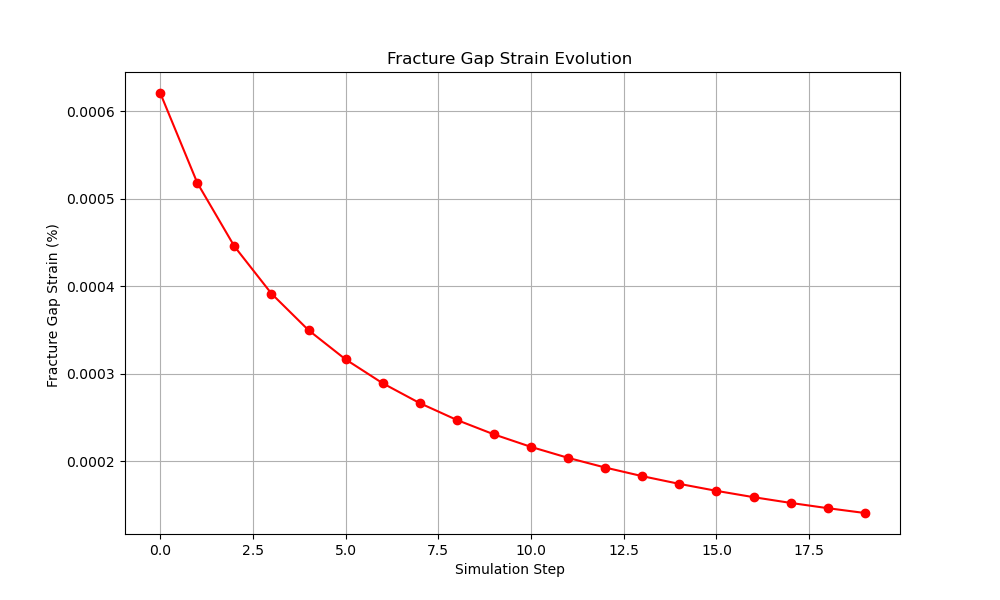
\includegraphics[width=0.7\textwidth]{../output_advanced/Flexible/gap_strain.png}
  \caption{Evolution of average fracture gap strain over simulation steps for the Flexible Fixator ($E_{fixator} = 35$ GPa).}
  \label{fig:flexible_gap_strain}
\end{figure}

\begin{figure}[htbp]
  \centering
  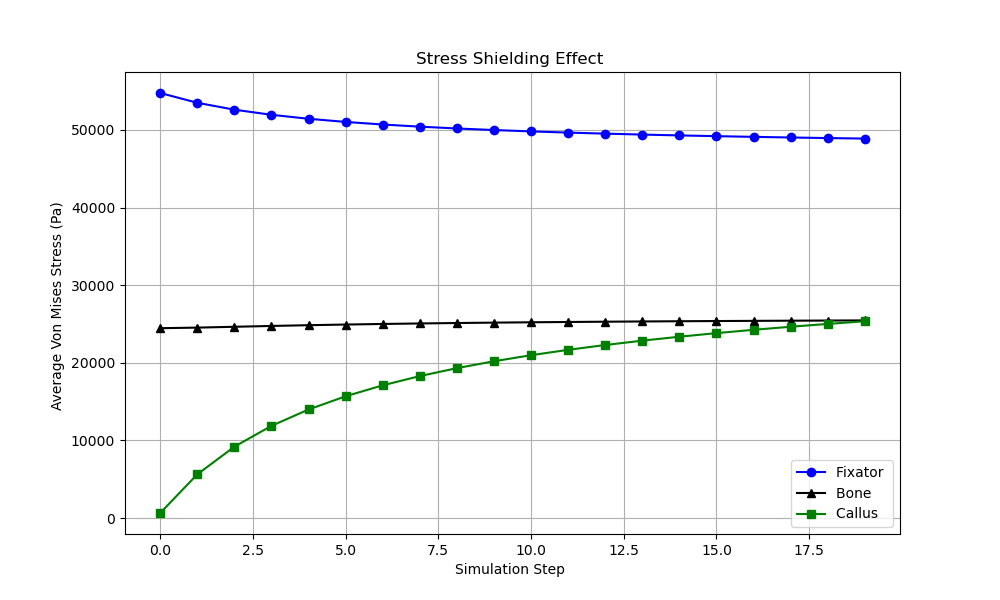
\includegraphics[width=0.7\textwidth]{../output_advanced/Flexible/stress_shielding.png}
  \caption{Evolution of average Von Mises stress in the fixator, bone, and callus regions for the Flexible Fixator ($E_{fixator} = 35$ GPa) over simulation steps, illustrating load sharing dynamics.}
  \label{fig:flexible_stress_shielding}
\end{figure}

% TODO: Add analysis, might delete clearpage
\clearpage % Ensures figures are placed before next major section

\subsubsection{Standard Fixator (\texorpdfstring{$E_{fixator} = 70$}{E\_fixator = 70} GPa)}

\begin{figure}[htbp]
  \centering
  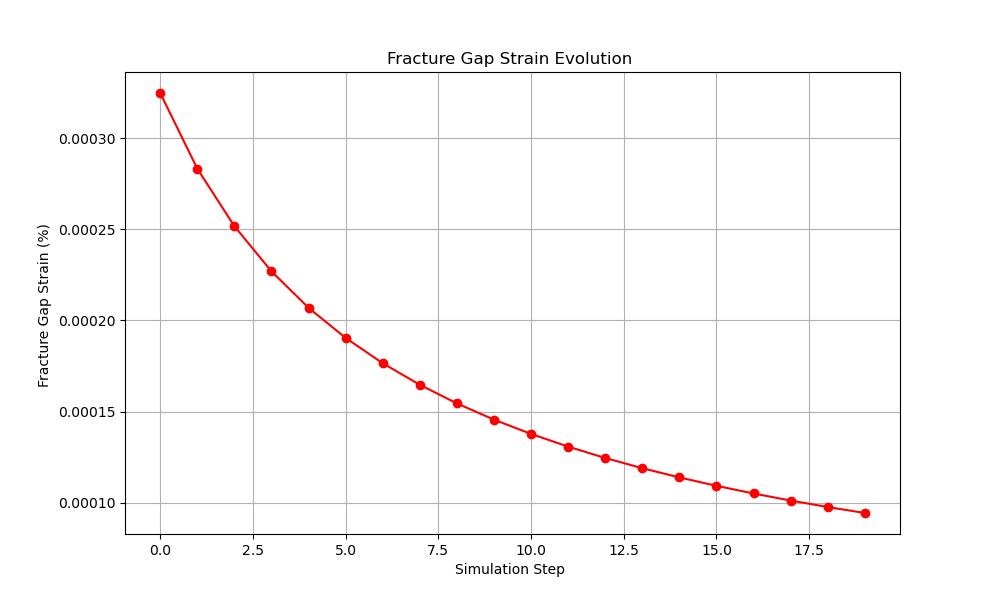
\includegraphics[width=0.7\textwidth]{../output_advanced/Standard/gap_strain.png}
  \caption{Evolution of average fracture gap strain over simulation steps for the Standard Fixator ($E_{fixator} = 70$ GPa).}
  \label{fig:standard_gap_strain}
\end{figure}

\begin{figure}[htbp]
  \centering
  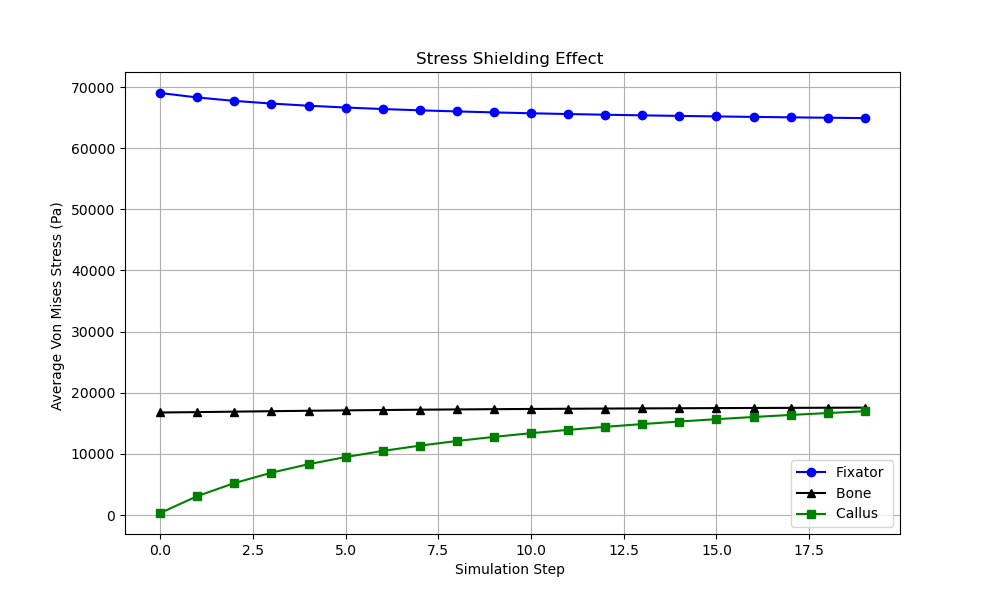
\includegraphics[width=0.7\textwidth]{../output_advanced/Standard/stress_shielding.png}
  \caption{Evolution of average Von Mises stress in the fixator, bone, and callus regions for the Standard Fixator ($E_{fixator} = 70$ GPa) over simulation steps, illustrating load sharing dynamics.}
  \label{fig:standard_stress_shielding}
\end{figure}

% TODO: Add analysis, might delete clearpage
\clearpage % Ensures figures are placed before next major section

\subsubsection{Rigid Fixator (\texorpdfstring{$E_{fixator} = 140$}{E\_fixator = 140} GPa)}

\begin{figure}[htbp]
  \centering
  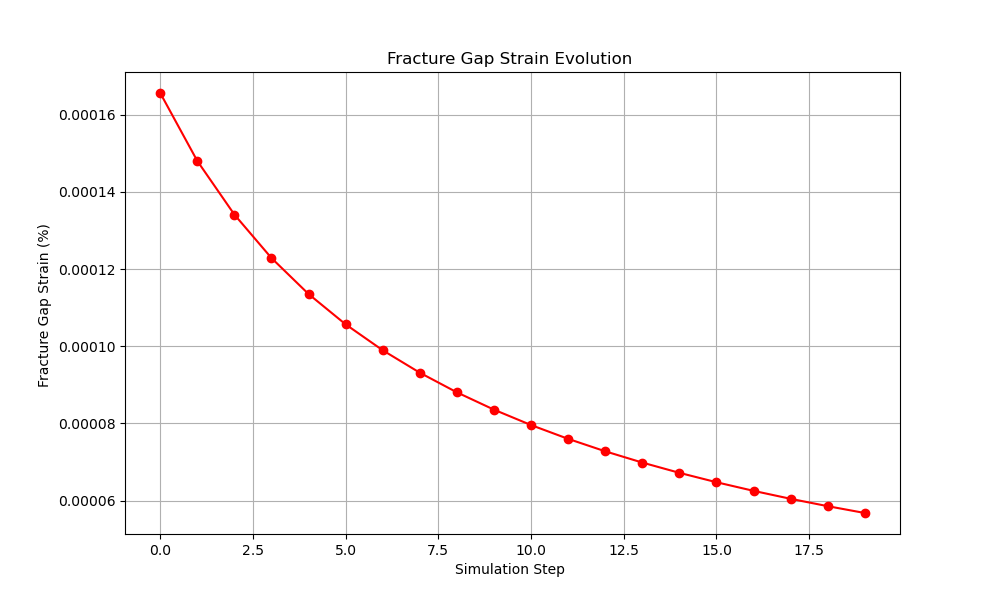
\includegraphics[width=0.7\textwidth]{../output_advanced/Rigid/gap_strain.png}
  \caption{Evolution of average fracture gap strain over simulation steps for the Rigid Fixator ($E_{fixator} = 140$ GPa).}
  \label{fig:rigid_gap_strain}
\end{figure}

\begin{figure}[htbp]
  \centering
  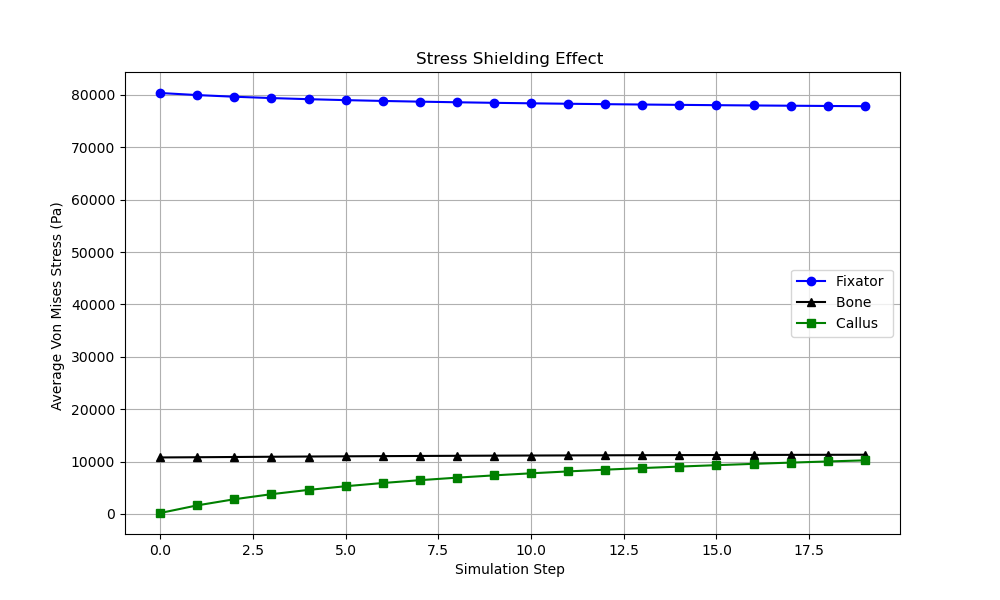
\includegraphics[width=0.7\textwidth]{../output_advanced/Rigid/stress_shielding.png}
  \caption{Evolution of average Von Mises stress in the fixator, bone, and callus regions for the Rigid Fixator ($E_{fixator} = 140$ GPa) over simulation steps, illustrating load sharing dynamics.}
  \label{fig:rigid_stress_shielding}
\end{figure}

% TODO: Add analysis, might delete clearpage
\clearpage

\section{Conclusion}
This project successfully developed and applied a 2D finite element model to simulate the biomechanics of fracture healing, specifically focusing on the influence of varying fixator stiffness. The parametric study yielded several key findings:
\begin{itemize}
  \item Increasing fixator stiffness consistently led to higher stress concentrations within the fixator itself, coupled with correspondingly lower stresses in both the bone and the healing callus. This quantitatively demonstrates the well-known phenomenon of stress shielding.
  \item More rigid fixators resulted in significantly lower average strains within the fracture gap (callus region) throughout the simulated healing process, indicating greater mechanical stability at the fracture site.
\end{itemize}
These observations are in strong agreement with established biomechanical principles governing fracture fixation and healing. The flexible fixator (35 GPa) facilitated greater load sharing with the bone and callus, which could potentially promote more vigorous and uniform callus formation under appropriate conditions. Conversely, the rigid fixator (140 GPa) provided maximum initial stability but also induced the most pronounced stress shielding, which might delay bone remodeling if prolonged. The standard fixator (70 GPa) exhibited an intermediate biomechanical response.

The Python-based simulation framework developed for this project provides a versatile and reusable tool for conducting such parametric FEA studies. It enables the generation of detailed stress contour maps, plots of stress and strain evolution over time, and comparative analyses across different design parameters. Figure \ref{fig:parametric_comparison} offers a concise visual summary of the principal differences observed across the three fixator types at the culmination of the simulated healing period.

Future research could build upon this foundation by extending the model to three dimensions (3D), incorporating more sophisticated material models for bone and callus (e.g., anisotropic, poroelastic, or viscoelastic properties), and integrating mechanobiological algorithms to directly simulate tissue differentiation and healing progression based on local mechanical stimuli. Nonetheless, the current 2D model serves as a valuable educational and investigative tool for understanding the fundamental interplay between fixator mechanics, stress transfer, and the evolving mechanical environment of a healing fracture.

\begin{figure}[htbp]
  \centering
  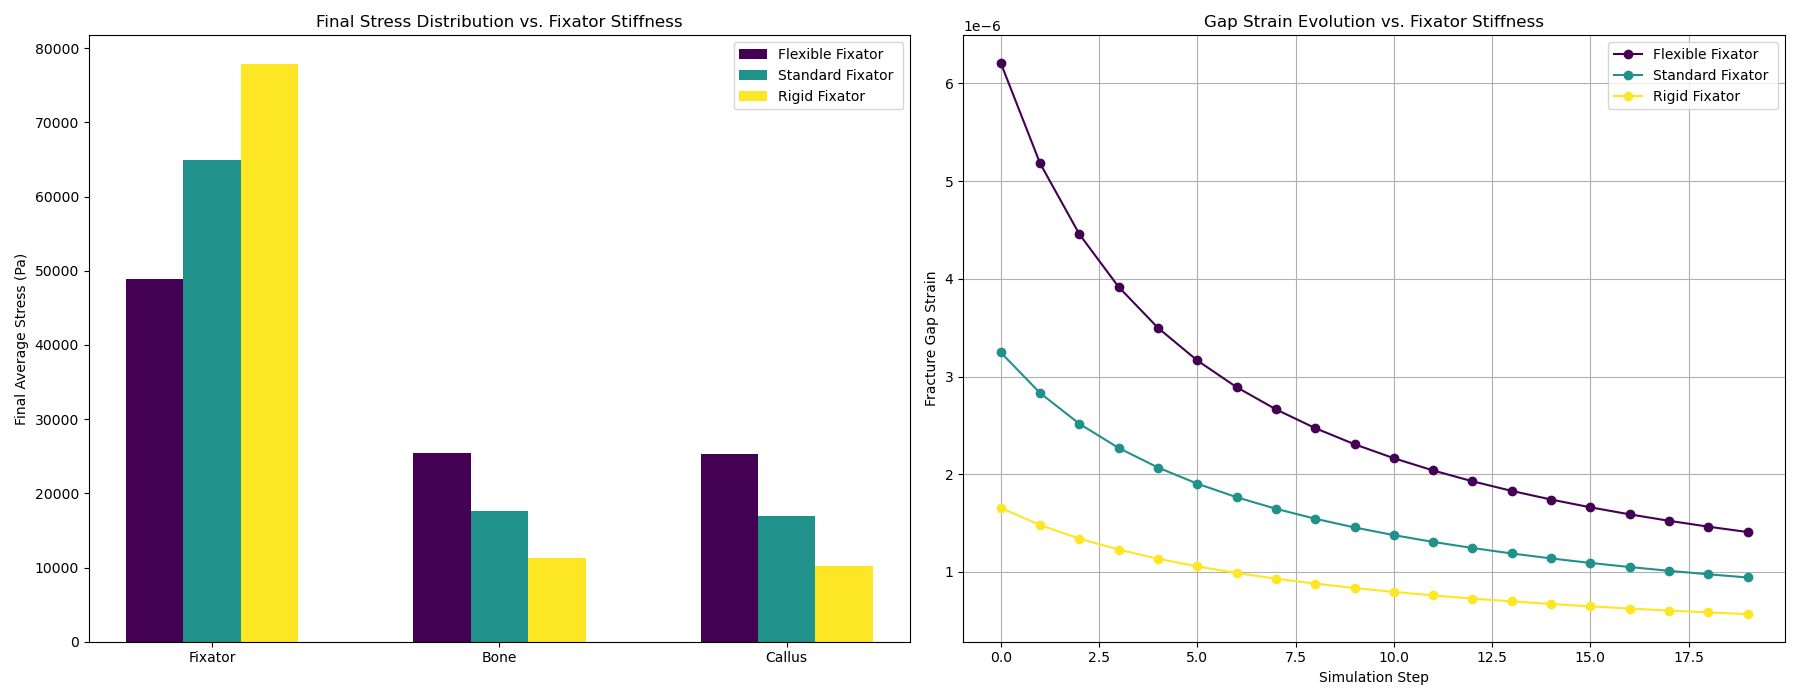
\includegraphics[width=0.95\textwidth]{../output_advanced/parametric_comparison.png}
  \caption{Parametric comparison across different fixator stiffnesses: (Left) Final average Von Mises stress distribution in the fixator, bone, and fully matured callus (Step 20). (Right) Evolution of average fracture gap strain over the 20 simulation steps for each fixator type.}
  \label{fig:parametric_comparison}
\end{figure}

\section{Appendix}

Student A: code of simulation, plot, 33$\%$ report writing

Student B: code of analysis, plot, 33$\%$ report writing

Student C: code of fea-core, plot, 33$\%$ report writing


%%%%%%%%%%%%%%%%%%%%%%%%%%%%%%%%%%%%%%%%%%%%%%%%%%%%%%%%%%%%%%%%%%%%%%%%%%%%%%%%%%
%%%%%%%%%%%%%%%%%%%%%%%%%%%%%%%%%%%%%%%%%%%%%%%%%%%%%%%%%%%%%%%%%%%%%%%%%%%%%%%%%%

% \section{Introduction}
% \lipsum[2]
% \lipsum[3]


% \section{Headings: first level}
% \label{sec:headings}

% \lipsum[4] See Section \ref{sec:headings}.

% \subsection{Headings: second level}
% \lipsum[5]
% \begin{equation}
% 	\xi _{ij}(t)=P(x_{t}=i,x_{t+1}=j|y,v,w;\theta)= {\frac {\alpha _{i}(t)a^{w_t}_{ij}\beta _{j}(t+1)b^{v_{t+1}}_{j}(y_{t+1})}{\sum _{i=1}^{N} \sum _{j=1}^{N} \alpha _{i}(t)a^{w_t}_{ij}\beta _{j}(t+1)b^{v_{t+1}}_{j}(y_{t+1})}}
% \end{equation}

% \subsubsection{Headings: third level}
% \lipsum[6]

% \paragraph{Paragraph}
% \lipsum[7]



% \section{Examples of citations, figures, tables, references}
% \label{sec:others}

% \subsection{Citations}
% Citations use \verb+natbib+. The documentation may be found at
% \begin{center}
% 	\url{http://mirrors.ctan.org/macros/latex/contrib/natbib/natnotes.pdf}
% \end{center}

% Here is an example usage of the two main commands (\verb+citet+ and \verb+citep+): Some people thought a thing \citep{kour2014real, hadash2018estimate} but other people thought something else \citep{kour2014fast}. Many people have speculated that if we knew exactly why \citet{kour2014fast} thought this\dots

% \subsection{Figures}
% \lipsum[10]
% See Figure \ref{fig:fig1}. Here is how you add footnotes. \footnote{Sample of the first footnote.}
% \lipsum[11]

% \begin{figure}
% 	\centering
% 	\fbox{\rule[-.5cm]{4cm}{4cm} \rule[-.5cm]{4cm}{0cm}}
% 	\caption{Sample figure caption.}
% 	\label{fig:fig1}
% \end{figure}

% \subsection{Tables}
% See awesome Table~\ref{tab:table}.

% The documentation for \verb+booktabs+ (`Publication quality tables in LaTeX') is available from:
% \begin{center}
% 	\url{https://www.ctan.org/pkg/booktabs}
% \end{center}


% \begin{table}
% 	\caption{Sample table title}
% 	\centering
% 	\begin{tabular}{lll}
% 		\toprule
% 		\multicolumn{2}{c}{Part}                   \\
% 		\cmidrule(r){1-2}
% 		Name     & Description     & Size ($\mu$m) \\
% 		\midrule
% 		Dendrite & Input terminal  & $\sim$100     \\
% 		Axon     & Output terminal & $\sim$10      \\
% 		Soma     & Cell body       & up to $10^6$  \\
% 		\bottomrule
% 	\end{tabular}
% 	\label{tab:table}
% \end{table}

% \subsection{Lists}
% \begin{itemize}
% 	\item Lorem ipsum dolor sit amet
% 	\item consectetur adipiscing elit.
% 	\item Aliquam dignissim blandit est, in dictum tortor gravida eget. In ac rutrum magna.
% \end{itemize}


\bibliographystyle{unsrtnat}
\bibliography{references}  %%% Uncomment this line and comment out the ``thebibliography'' section below to use the external .bib file (using bibtex) .


%%% Uncomment this section and comment out the \bibliography{references} line above to use inline references.
% \begin{thebibliography}{1}

% 	\bibitem{kour2014real}
% 	George Kour and Raid Saabne.
% 	\newblock Real-time segmentation of on-line handwritten arabic script.
% 	\newblock In {\em Frontiers in Handwriting Recognition (ICFHR), 2014 14th
% 			International Conference on}, pages 417--422. IEEE, 2014.

% 	\bibitem{kour2014fast}
% 	George Kour and Raid Saabne.
% 	\newblock Fast classification of handwritten on-line arabic characters.
% 	\newblock In {\em Soft Computing and Pattern Recognition (SoCPaR), 2014 6th
% 			International Conference of}, pages 312--318. IEEE, 2014.

% 	\bibitem{hadash2018estimate}
% 	Guy Hadash, Einat Kermany, Boaz Carmeli, Ofer Lavi, George Kour, and Alon
% 	Jacovi.
% 	\newblock Estimate and replace: A novel approach to integrating deep neural
% 	networks with existing applications.
% 	\newblock {\em arXiv preprint arXiv:1804.09028}, 2018.

% \end{thebibliography}


\end{document}
